\documentclass[12pt]{article}
\usepackage[utf8]{inputenc}
\usepackage[T1]{fontenc}
\usepackage{graphicx}
\usepackage{xcolor}
\usepackage{hyperref}
\usepackage[english]{babel}

%%novalidate

\usepackage{tikz}
\usepackage{calc}
\usepackage{booktabs}
%\usepackage{hyperref}

% colors
\definecolor{color1}{HTML}{000060}
%\definecolor{color1}{HTML}{8C260F}
\definecolor{color2}{HTML}{333333}


% fonts
\usepackage{fontspec}
\defaultfontfeatures{Mapping=tex-text}
\setmainfont
[BoldFont=Lato-Bold.ttf,
ItalicFont=Lato-Italic.ttf,
BoldItalicFont=Lato-BoldItalic.ttf]
{Lato-Regular.ttf}
\newfontfamily\headingfont[ItalicFont=Lato-BlackItalic.ttf]{Lato-Black.ttf}
%%%

\usepackage{geometry}
\geometry{a4paper,
hmargin=20mm,vmargin=20mm,
head=0ex,foot=3ex}

\linespread{1.3}

\usepackage[hang]{caption}
\DeclareCaptionFormat{upper}{#1#2\uppercase{#3}\par}
\captionsetup{labelfont={bf,color=color2},textfont={normalsize,color=color2},format = upper,figurename=FIGURE,tablename=TABLE}

%%% fancy sections
\usepackage{titlesec}
%\titleformat{\chapter}{\headingfont\LARGE\bfseries\scshape\color{color1}}{\thechapter}{1em}{}[\titlerule]
\titleformat{\section}{\color{color1}\headingfont\Large\bfseries\uppercase}{\thesection}{1em}{}[\titlerule]
\titleformat{\subsection}{\color{color1}\headingfont\large\bfseries\uppercase}{\thesubsection}{1em}{}
\titleformat{\subsubsection}{\color{color1}\headingfont\bfseries\uppercase}{\thesubsubsection}{1em}{}
%%%

% head and foot
\usepackage{fancyhdr}
\pagestyle{fancy}
\lhead{}
\chead{}
\makeatletter
\rhead{\color{color2}\@date}
\makeatother
\newlength{\myheight}
\lfoot{
\settoheight{\myheight}{\thepage}
\raisebox{-2ex-0.5\myheight}{
\includegraphics[height=4ex]{logo}}
}
\cfoot{\color{color2}VIET NGUYEN - Aalto University}
\rfoot{\color{color2}\thepage}
\renewcommand\headrulewidth{0pt}
\renewcommand\footrulewidth{0pt}

%%% picture on cover page
\usepackage{eso-pic}
\newcommand\BackgroundPic{%
\put(0,0){%
\parbox[b][\paperheight]{\paperwidth}{%
\vfill
\centering

\includegraphics[width=\paperwidth,height=\paperheight,%
keepaspectratio]{cover}%
\vfill
}}}
%%%
% custom titlepage
\makeatletter
\renewcommand{\maketitle}{
\thispagestyle{empty}
\AddToShipoutPicture*{\BackgroundPic}
\ClearShipoutPicture
%
\phantom{a}
\vfill
\phantom{a}\hfill
\begin{tabular}[c]{@{}p{0.7\textwidth}@{}}
      \color{white}\headingfont\LARGE\@title\\[1em]
      \color{white}\headingfont\Large\@author\\[2em]
\end{tabular}
%
\clearpage
}
\makeatother
%%%


%%% fancy boxes
\usepackage{tcolorbox}
\usepackage{wrapfig}
\def\fullboxbegin{
\bigskip
\begin{tcolorbox}[colback=color1,colframe=color1,coltext=white,arc=0mm,boxrule=0pt]
}
\def\fullboxend{\end{tcolorbox}\medskip}
%
\def\leftboxbegin{
\begin{wrapfigure}{l}{0.5\textwidth}
\begin{tcolorbox}[colback=color1,colframe=color1,coltext=white,arc=0mm,boxrule=0pt]
}
\def\leftboxend{
\end{tcolorbox}
\end{wrapfigure}
}
%
\def\rightboxbegin{
\begin{wrapfigure}{r}{0.5\textwidth}
\begin{tcolorbox}[colback=color1,colframe=color1,coltext=white,arc=0mm,boxrule=0pt]
}
\def\rightboxend{
\end{tcolorbox}
\end{wrapfigure}
}
%
\newcounter{frames}
\def\frameboxbegin#1{
\bigskip
\refstepcounter{frames}
\begin{tcolorbox}[colback=white,colframe=color1,arc=0mm,title={\MakeUppercase{\textbf{Frame \arabic{frames}}: #1}}]
}
\def\frameboxend{
\end{tcolorbox}
}
%%%

\usepackage{lipsum}
\usepackage[nottoc]{tocbibind}

%%%%%%%%%%%%%%%
% Title Page
\title{Application of blockchain in telecom industry}
\author{Viet Nguyen \newline Aalto University}
\date{}
%%%%%%%%%%%%%%%

\begin{document}
\maketitle

\tableofcontents
\clearpage

\section{Introduction}

\noindent

Blockchain is currently one of the most talked-about technologies. Across industries, organizations
are exploring blockchain’s potential impact in their space and how they can benefit from
this emerging technology. The telecommunications industry is no exception

So what is the benefit of blockchain ? The
core attributes of blockchain’s shared ledger approach help provide trust, security, transparency
and control across the participating ecosystem for all points in a transaction process.
This results in the potential for lower costs, faster throughput and improved experiences for all
players

\subsection{What is a blockchain?}

The advantages of this type of multiple,
decentralized storage are robustness and
trust, at the expense of confidentiality and
processing performance. Every participant
in the network has the ability to verify
the correctness of transactions. Network
consensus methods and cryptographic
technology are used to validate transactions.
Thus, trust is not established
externally by a central authority or an
auditor but continuously within the network
as illustrated in Figure 1. Furthermore,
decentralized storage in blockchains is
known to be very failure-resistant. Even in
the event of the failure of a large number of network participants the blockchain
remains available, eliminating the single
point of failure. New information stored in
the blockchain is immutable. Its method
of record-keeping prevents deletion or
reversing of transactions once added to the
blockchain, as soon as further blocks are
added. 

\includegraphics[width=1\textwidth]{"fig1.jpg"}

A blockchain’s key characteristics as
illustrated in Figure 2 are integral to its
potential.

\includegraphics[width=1\textwidth]{"fig2.jpg"}

\section{CSP value chain and blockchain}

Communications service providers (CSPs)
have traditionally owned the end-to-end telecoms
value chain for both consumers and
businesses – spanning network infrastructure,
provision of core voice and data connectivity,
and related consumer services.
However, in an environment of heightened
competition in an increasingly digital world
from infrastructure light over the top (OTT)
players, together with decreasing revenues
from voice and increasing costs due to the
high band-width demands, there is a need to both reduce costs and find new sources
of revenue

Blockchain has the potential to be for ‘value’
what the Internet has been for ‘information’.
In addition to the many use cases being
explored for industries such as finance,
healthcare, and government, there are
plausible applications of blockchain for a
CSP, both within its current portfolio of
operations and also to capitalize on some of
the future telecom trends.

\includegraphics[width=1\textwidth]{"fig3.jpg"}

CSPs will most probably see the greatest
impact of blockchain in their core
management systems and in adjacent
services, providing opportunities for cost
reduction through process efficiency gains,
and revenue growth through new value propositions. Four use cases help illustrate
the potential of blockchain for CSPs: Fraud
Management, Identity-as-a-service and
Data Management, 5G enablement, and
secure IoT connectivity

\includegraphics[width=1\textwidth]{"fig4.jpg"}

\section{Use Case - Fraud Prevention}

Fraud detection and prevention continue
to be topics of relevance for most CSPs,
as a result of fraud costs in the industry of
over USD 38 billion11 annually. Given that
the telecoms industry has not yet found a
way to effectively and sustainably prevent
fraud, blockchain is in principle a good
contender for significantly decreasing the
cost of fraud e.g. in roaming and in identity
management. 

\subsection{Roaming fraud}
Current system - When a call/event is
placed, the Visited Public Mobile Network
(VPMN) queries the Host Public Mobile
Network (HPMN) about the services to
which the roaming user has subscribed,
by querying the Home Location Register
(HLR). The Call Detail Records (CDRs) are
sent to the billing systems in their respective
networks. These systems are in charge
of processing CDRs and the generation of
invoices to subscribers.

The VPMN sends CDR information to the
HPMN as a Transfer Account Procedure
(TAP) file. Certain companies act as a Data
Clearing House (DCH) for these files. A DCH
is responsible for the transmission and
conversion of the TAP files on behalf of the
CSP which has hired it.

Once the TAP files are received, the HPMN
must settle accounts per costs incurred with the VPMN in accordance with the corresponding roaming agreement tariffs.

\leftboxbegin
Blockchain has the
potential to reduce losses
due to fraud and minimize
costs for fraud detection
applications.
\leftboxend

Current challenges – Roaming fraud occurs
when a subscriber accesses the resources
of the HPMN via the VPNM but the HPMN
is unable to charge the subscriber for the
services provided, but is obliged to pay the
VPNM for the roaming services. Roaming
fraud exploits two characteristics:
\begin{itemize}
	\item Longer detection time: since the fraud occurs
	when the subscriber is in a network
	other than that of the HPMN, the time
	required to detect the fraud is longer
	due to delays in the exchange of data
	between VPMN and HPMN.
	\item Longer response time: due to lack of control over the systems in which the fraud
	has occurred, the time to respond to the
	fraud is longer than if the fraud had occurred
	in a system owned by the HPMN.
\end{itemize}

\begin{figure}[!h]
\centering
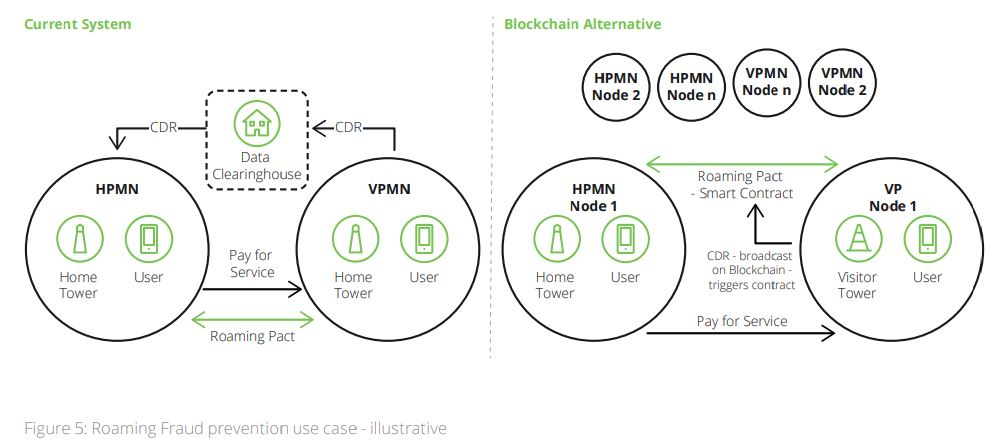
\includegraphics[width=0.5\textwidth]{fig5.jpg}
\end{figure}

\subsubsection{Blockchain-based solution}
A permissioned blockchain could
be implemented between every
pair of operators which have a roaming
agreement. Designated nodes from both
operators act as miners to verify the sanctity
of each transaction broadcasted on the
network. The roaming agreement is implemented between the HPMN and the VPMN
as a smart contract that is triggered when
a transaction containing the CDR data is
broadcasted on the blockchain network.
Every time a subscriber triggers an event
in a visiting network, the VPMN broadcasts
the CDR information as a transaction to
the HPMN. This data triggers the smart
contract and the terms of the agreement
are executed. The HPMN can thus automatically calculate the billing amount based
on the services rendered and send this
information back to the VPMN.
This helps instantaneous and verified authorization as well as settlement to occur in
line with blockchain-based smart contract
terms. CSPs can also do away with the DCH
acting as middleman, resulting in further
cost savings



\subsection{Subscription identity fraud}
\subsubsection{Current system}



\noindent  Subscriber identity information is necessary to create an account
and assign services to the subscriber.
Subscription ID theft occurs when a subscriber uses false identification or another
subscriber’s (victim) ID to obtain services.
Fraudsters can for example use the stolen
identity information to obtain a SIM card in
the victim’s name.
\leftboxbegin
Benefit
\begin{itemize}
	\item Cost savings from eliminating the
	third-party clearing house
	\item Automatic triggering of roaming
	contract based on call/event data
	which enables near-instantaneous charging and reduction in
	roaming fraud
	\item Repository of verifiable transactions
	between operators, allowing
	for quick dispute resolution.
\end{itemize}
\leftboxend

\noindent The physical SIM stores the International
Mobile Subscriber Identity (IMSI) and the
related key is used to identify and authenticate subscribers on mobile devices.
Each time a mobile device is turned on, it
broadcasts a signal containing the IMSI to
the nearest base station. That identification
number links the device to the account with
the carrier

\noindent Some telecom providers maintain their
own fraud databases to identify potential
fraud activities. Current solutions are either weak (CSP asks customers to create passcode while creating a wireless account) or
expensive (stand-alone ID protection
systems such as Equifax), and are sometimes not up-to-date. 
\begin{figure}[!h]
	\centering
	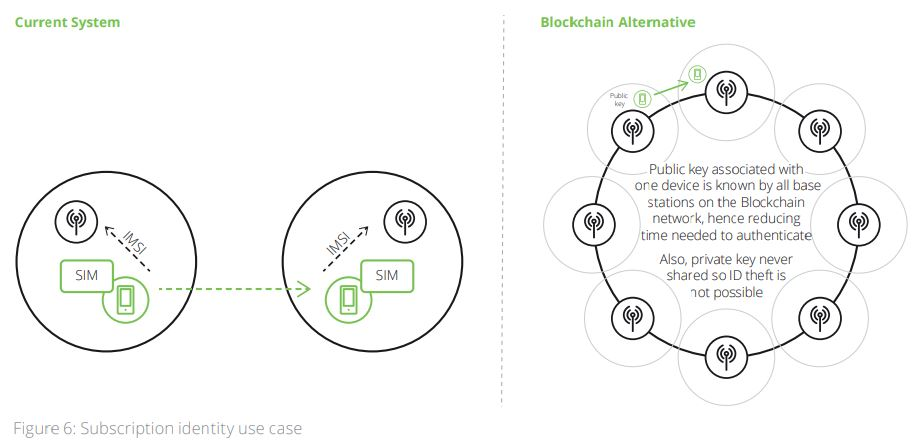
\includegraphics[width=0.5\textwidth]{fig6.jpg}
\end{figure}
\subsubsection{Current challenges}
There are many ways
in which a subscriber’s identity can be compromised (email phishing, SIM cloning, etc.).
Due to the multiple-play services provided
by telecom operators, an ID theft can result
in compounded losses through the access
to many services under a stolen identity.


\subsubsection{Blockchain-based solution}

Public-private cryptography
which is inherent in a blockchain
can be used to identify a device and link
that device to a subscriber’s identity.
Instead of broadcasting the IMSI to the network to identify the device, the phone-generated public key is broadcasted instead.
The device generates this public key from
the private key that is stored securely on
it. Neither the carrier nor any other third
party needs to know the private key.

\rightboxbegin
Benefit
\begin{itemize}
	\item Reduced subscriber or other ID-based
	fraud. 
	\item Easier and faster device identification during mobility, due to shared
	database having the device public
	key information and history.
	\item Can be used to provide identity to
	machines in an M2M or broader
	IoT environment, instead of having to embed physical SIMs into
	distributed devices.
	\item Elimination of cost to manufacture
	and distribute physical SIMs.
\end{itemize}
\rightboxend

This ‘eSIM’ solution can help protect private
information that is encrypted in the private
key. The private key is associated with only
one particular device and is hence difficult
to steal. The public key is used to identify
the device and to authorize it on the network. The subscriber is uniquely identified
by this public key, while able to keep the private key information secret. This way, the
services can only be used by the subscriber
who has subscribed to them and the ID
cannot be easily stolen.

This process also avoids the device information having to be authenticated by the
base station every time the device enters a
new cell territory. Instead, due to the base
stations being nodes on a common blockchain, the device information is already
available at the base station and can be
authenticated quickly, once the public key
is sent to it by the device.

\section{Use Case - Identity-as-a-service and Data Management}

CSPs can create new sources of revenue by
providing identity and authentication as well
as data management solutions to partners,
enabled by a blockchain.

\leftboxbegin
Blockchain adoption
could significantly reduce
roaming fraud and also
optimize ID management
through instantaneous
and automated processes
based on smart contracts.
\leftboxend

Currently, every time a person wants to
sign up at a vendor, they need to prove
their identity and credentials using physical
or digital documents. They would need to
provide their PII (Personal Identity Information)
even though most of the information
would not be needed by every vendor; the
vendor would only need a subset of that
information. Also, signing up online either
requires creating many username/password
combinations or utilizing the services of
third party providers (such as Google and
Facebook) to use their SSO (Single Sign On)
functionalities.

This leads to many challenges such as lack
of convenience (many username/ password
combinations) and security (personal data
shared with third parties) in current identity
and authentication services. And while
there are a few alternatives, CSPs currently
do not play a significant part in identity and
authorization services, even though they
possess substantial amounts of relevant
subscriber data.

\textbf{Opportunity for CSPs}

A blockchain can be used as the shared
ledger that stores identity transactions. The
CSP can provide identity-as-a-service to
partners, thus allowing for additional revenue
generation by negotiating appropriate
agreements.

When a subscriber opens an account with a
CSP, the CSP creates a digital identity. The
private key associated with this identity is
stored safely on the eSIM. The CSP creates
a virtual identity, using the public key from
the digital identity and adds a set of standard
fields (name, address, etc.) as required.
It then adds a digital signature using its
own private key. A pointer to this virtual
identity along with necessary descriptors is
then added to the blockchain.

If the subscriber now visits a partner
website, say an e-commerce site, the site
will need to know their identity, so the
merchant site starts running the corresponding
app on the phone to provide
the identity. A copy of the ledger entry is
sent to the e-commerce site app. Now the
e-commerce app can look at all entries for
that same virtual identity. Once the virtual
identity is established, the e-commerce
site needs to know that the virtual identity
belongs to the subscriber so its app takes
the public key from the virtual identity,
encrypts a challenge and sends it to their
app which decrypts it (because it has the
associated private key) and responds. Now
the e-commerce site generates an e-commerce
virtual identity which is then stored
in the ledger itself.

The next time the subscriber visits the
same e-commerce site, he can be authenticated
using the same mechanism. Also, the
ledger already holds his transaction history
and hence knows his preferences. The
e-commerce site can use related insights
for a recommendation engine. The subscriber
can also use the same e-commerce
virtual identity to login to a completely
different e-commerce site using the same
mechanism.

The CSP virtual identity can be used to help
create further virtual identities similar to the
e-commerce one (such as a travel virtual
identity). This identity need not know all
of the details from the subscribers digital
identity, only the ones that are relevant
(such as his home location) and add other
attributes (such as his preferred mode of
travel) to create a travel virtual identity. The
possibilities of such identity management
are limited only by the number of partner
service providers that the CSP can sign on
to the blockchain-based system.

\frameboxbegin{Benefits}
\begin{itemize}
\item Cost savings from a blockchainbased
federated identity
management solution as
compared to traditional IDM
software.
\item New revenue stream from
providing an identity-as-a-service
solution to partners and endconsumers.
\item Improved subscriber ease of use
as regards ID management.
\item Opportunity to form a locked-in
ecosystem through strategic
partnerships with partners that
use identity solutions provided by
the CSP.

\end{itemize}
\frameboxend

\subsection{Application to Data Management}
The CSP can extend such a blockchain-enabled
identity and access solution to provide
data storage and verification services to
private clients. Consider the example of
an educational institution. Educational
institutions issue certificates and degrees
to their students to signal the completion
of a course. The current system of managing
certificates is slow, unreliable, and
disjointed. It often still requires maintaining
a paper copy of the certificate to be physically
submitted to third parties legitimately
requesting proof of course completion
and grades. Additional steps today might
include an employer, for example, calling a
university to verify that a certificate is not a
fake, or relying on a third-party to perform
that verification.

CSPs could provide blockchain based
Identity verification, data management and
storage services to both private clients and
subscribers, generating additional revenue
in the process. The educational institution
signs up with the CSP to digitize and store
certificates of subscribers on the blockchain.
For those subscribers who also sign
up (and are, of course, alumni of the university),
their identity and degree certificate are
verified by the university through traditional
channels, and the university assigns the
digital copy of that certificate along with all
details (course name, date of issue, etc.) to
the subscriber.

If a prospective employer of the subscriber
now wants to verify the credentials and
inspect the certificate, the subscriber only
needs to produce the digital certificate available
on the blockchain and the employer
can be sure that this has been issued by
the university and is genuine. The CSP can
further benefit by extending related authentication
services to corporate clients for all
types of documents, such as insurance certificates,
airline tickets, hotel reservations,
etc., where digital storage and verification
may be required at some point.

\section{Use Case - 5g enablement}
5G technology implementation is another
example to potentially benefit from the
blockchain to streamline processes. To
realize the 5G promise of ubiquitous access
across various networks, CSPs will need
to handle heterogeneous access nodes
and diverse access mechanisms. Selecting
the fastest access node for every user
or machine will be a central challenge in
the future. Blockchain can enable a new
generation of access technology selection
mechanisms to build sustainable solutions.

Current system – ANDSF, which stands for
Access Network Discovery and Selection
Function, is an entity within the EPC
(Evolved Packet Core) which helps in the
discovery/selection of access networks,
such as WiFi, WiMax, and LTE, in the device
vicinity, providing them with rules policing
the connection to these networks. It consists
of a list of access networks, such as
WiFi, that may be available in the vicinity of
a device. This information is received in response
to a device request which contains
its location and capability, such as types of
supported interfaces, among others. The
received information assists the device in
expediting connection to these networks.
The ANDSF response contains the following
information: the type of access
technology (WiFi, WiMAX, etc.), the access
network identifier, and technology-specific
information (such as one or more carrier
frequencies).
Current challenges – The system is centralized
in a client-server model where the
rules stored on the server (ANDSF) are
pushed to the client (device). This causes
delays and does not allow for seamless
provisioning between access networks for
the device. Also, the provisioning of rules is
not a real-time process – meaning the rules
cannot be changed dynamically.

\frameboxbegin{Benefits}
\begin{itemize}
	\item Sharing of faster and regulated
	local connectivity for reliable
	service to device.
	\item Instant monetization of diverse
	connection types through smart
	contracts.
	\item Enables local connection prices
	purely based on supply and
	demand in the area.
	\item New business models to use idle
	capacity for non-prioritized traffic.
	
\end{itemize}
\frameboxend
\subsection{Blockchain-based solution}
The 3GPP (LTE, GPRS) and
non-3GPP (WiMax, WLAN, WiFi)
access networks in a given area can be networked
via a blockchain where each access
point (WiFi router, SP cell tower, etc.) can
serve as a node in the network monitoring
the devices.
Rules and agreements between the various
access providing networks can be coded
as smart contracts. These contracts can be
dynamic in nature wherein any time a policy
needs to be changed, only the contract
code needs to be changed.
When a device broadcasts its identity,
it is accepted into the network by the
corresponding CSP cell. Once the device
broadcasts its location, the access node
that can best provide service to the device
is called upon to do so.
This also allows for seamless rating and
charging of all services between the various
access nodes. If, for example, a WLAN
from an office or a home network has
provided access to a device, then the CSP
can conceivably give a reduction in the bill
amount appropriately for the invoice of the
accommodating company or home. Location-
based services can also be enabled by
being a part of this blockchain network and
hence always knowing which devices are in
Figure 7: Identity-as-a-Service and Data Management use case the vicinity.
\section{Use Case - IoT connectivity}
A blockchain can enable secure and
error free peer-to-peer connectivity for
thousands of IoT devices with cost-efficient
self-managed networks. For example,
machines within a manufacturing plant will
be able to communicate and authenticate
themselves via the blockchain to steer
production processes. Active manual intervention
by the workforce will for example
only be needed if individual machines
require service on the basis of predictive
maintenance indicators. In addition, the
risk of a production shut-down owing to
corrupted or hacked machines could be
limited, thanks to the distributed and consensus-
based authentication of data in the
blockchain network.
Current system – To cope with the increased
connectivity demand for devices
with low-power consumption, traffic, and
bandwidth needs, current network operators
build Low Power Wide Area Networks
(LPWAN). Telcos are facilitating appropriate
IoT use cases for regionally and globally
operating companies to push and fully
amortize LPWANs. These use cases often
require appropriate platforms to manage
single IoT devices and connect the internal
application landscapes accordingly.
Current challenges – IoT sensors usually
carry sensitive information about core assets
or in some way pertaining to customers
of the company, which makes data and
network security an essential and costly
pillar of IoT connectivity. Also, the size of
the network defines network routing and
management complexity, leading to varying
system landscapes without a common
platform.

\frameboxbegin{Benefits}
\begin{itemize}
	\item Self-managed, peer-to-peer
	networks taking over regional
	routing.
	\item High security levels for IoT devices
	within public blockchain networks.
	\item Low-cost setup options for SME
	purposes.
	
\end{itemize}
\frameboxend

\subsection{Blockchain-based solution}
A blockchain allows for highly
secure peer-to-peer self-managed
mesh networks using a sufficiently
large number of nodes. These blockchain
network nodes can be represented by
single embedded IoT sensors with the
ability to verify every block being changed
within the blockchain. For a start, these
networks can be introduced into a private
environment based in mid-range cell-towers
with relatively low investment requirements.
By establishing such a network in a
public blockchain language (e.g. Bitcoin or
Ethereum), further expansion or evolution
into a public blockchain enables seamless
connectivity and security. CSPs could then
provide private/public key security and
global, always-on connectivity to enable
such a public blockchain network with
global reach.
\section{Benefits, challenges and conclusion}
\subsection{Benefits:}
\begin{itemize}
	\item A blockchain’s ‘enabled’ trust improves
	coordination between various
	partners, due to a shared view of
	transactions and liabilities. This in
	turn permits the elimination of third
	parties, resulting in cost savings.
	\item Facilitates a single view of data instead
	of the need for consolidation across
	various disparate systems. Also allows
	for reliable audit trails due to the history
	of all transactions being available in
	the ledger.
	\item Implementation of smart contracts
	in roaming and other cases allows for
	near-instantaneous charging, thus
	leading to improved revenue assurance
	and fraud reduction.
	\item Potential to facilitate new business
	models for revenue generation for
	Communication Service Provider
	who are looking for new avenues to
	increase both top and bottom lines.
	\item A blockchain can act as the ledger
	that enables, for example, an M2M
	economy to prosper based on the
	common platform available, in which
	M2M transactions can be recorded. It
	can thus act as the enabler for an IoT
	ecosystem.
\end{itemize}
\subsection{Challenges:}
\begin{itemize}
	\item Since a blockchain retains all historical
	data, the size of an established blockchain
	at each node might become
	unsustainable. Instead, a mechanism
	to archive historical data needs to
	be looked at. Several alternatives are
	currently being explored in this regard
	by various players in the blockchain
	ecosystem.
	\item Conforming to existing data standards
	in terms of both structure and transport
	for sharing of information could
	prove to be an initial hurdle.
	\item Clear regulatory frameworks need to
	be defined for the implementation of
	agreements as digital, smart contracts
\end{itemize}
\subsection{Conclusion:}
In conclusion, the benefits of adopting
a blockchain in the core and auxiliary
operations of a Communications Service
Provider are plenty, as highlighted above.
CSPs should take a long term view of
blockchains and their potential to add value
to the enterprise in both their current and
new business models.

There will be challenges to adoption of the
blockchain, as with any new technology
that holds the promise of significant
disruption. However, CSPs would do well to
work together to enable the full realization
of the benefits, just as many of the global
financial institutions are currently doing
(e.g. in the R3 Consortium). Working in a
silo will limit the potential of blockchain,
as disintermediation, robustness, and
the need for trust at the intersection
of many stakeholders drives real value.
Organizations such as the GSMA, which
represents the interests of many mobile
CSPs globally, could equally take a more
active role in exploring and promoting
blockchain use cases in the industry.

Companies such as Orange and Verizon,
amongst others, have already invested
in startups in the blockchain area to
explore the synergies and potential use
cases. Many more players are researching
potential use cases in-house. It is time for
everyone to agree on a unified approach to
enable meaningful realisation of benefits.
%\section{Features commands}
%
%\subsection{Pictures used}
%
%\noindent
%Cover picture filename (in titlepage): \texttt{cover}\\
%Logo filename (in foot): \texttt{logo}
%
%\subsection{Boxes}
%
%\begin{verbatim}
%\fullboxbegin
%Content
%\fullboxend
%\end{verbatim}
%
%\begin{verbatim}
%\leftboxbegin
%Content
%\leftboxend
%\end{verbatim}
%
%\begin{verbatim}
%\rightboxbegin
%Content
%\rightboxend
%\end{verbatim}
%
%\begin{verbatim}
%\frameboxbegin{Frame Title}
%Content
%\frameboxend
%\end{verbatim}
%
%\newpage
%
%\section{First section}
%\lipsum[1]
%
%\fullboxbegin
%\lipsum[1]
%\fullboxend
%
%\lipsum[1]
%
%\subsection{First subsection}
%\lipsum[1]
%
%\leftboxbegin
%Lorem ipsum dolor sit amet, consectetuer adipiscing elit. Ut purus elit, vestibulum ut, placerat ac, adipiscing vitae, felis. Curabitur dictum gravida mauris. Nam arcu libero, nonummy eget, consectetuer id, vulputate a, magna. Donec vehicula augue eu neque. 
%\leftboxend
%
%\lipsum[1-2]
%
%\rightboxbegin
%\begin{itemize}
% \item Lorem ipsum
% \item Lorem ipsum
%\end{itemize}
%\rightboxend
%
%\lipsum[1]
%
%\subsubsection{First subsubsection}
%
%This document is an example of BibTeX using in bibliography management. Three items are cited: \textit{The \LaTeX\ Companion} book \cite{latexcompanion}, the Einstein journal paper \cite{einstein}, and the Donald Knuth's website \cite{knuthwebsite}. The \LaTeX\ related items are \cite{latexcompanion,knuthwebsite}.
%
%
%\begin{figure}[!h]
%\centering
%\includegraphics[width=0.5\textwidth]{sky.jpg}
%\caption{The sky is the limit.}
%\end{figure}
%
%\section*{Unnumbered section}
%\lipsum[1]
%
%\begin{figure}[!h]
%\centering
%\includegraphics[width=0.5\textwidth]{sky.jpg}
%\caption*{The sky is the limit.}
%\end{figure}
%
%\section{Second section}
%
%\lipsum[1]
%\begin{table}[!h]
%\centering
%\caption{Sample table.}
%\begin{tabular}{cccc}
%\toprule
%Value 1 & Value 2 & Value 3 & Value 4\\
%\midrule
% odd     & odd   & odd & 1.00 \\
% even    & even  & even& 1.00 \\
% odd     & odd   & odd & 1.00 \\
% even    & even  & even& 1.00 \\
%\bottomrule
%\end{tabular}
%\end{table}
%
%\lipsum[1]
%
%\frameboxbegin{Sample frame}
%\lipsum[1]
%\frameboxend
%
%\bibliographystyle{unsrt}
%\bibliography{sample}
\end{document}          
